% !Mode:: "TeX:UTF-8"
% !TEX program  = xelatex
\documentclass{sdureport}

% no head line or foot line
%\pagestyle{empty}

% just for filling a few pages
\usepackage{blindtext}
\usepackage{ctex}
\usepackage{indentfirst}
\usepackage{booktabs}
\usepackage{amsmath}
\usepackage{anyfontsize} % 公式字体报错问题

% 列表间距过大
% \usepackage{paralist}
% \let\itemize\compactitem
% \let\enditemize\endcompactitem
% \let\enumerate\compactenum
% \let\endenumerate\endcompactenum
% \let\description\compactdesc
% \let\enddescription\endcompactdesc

% initialize the variable texts
\sduCollege{计算机科学与技术}
\sduCourse{机器学习(双语)}
\sduSdudentId{202012345678}
\sduName{你的姓名}
\sduClass{你的班级}
\sduExperimentalTopics{实验1\  线性回归}
\sduExexperimentalHours{2h}
\sduDate{\today}

\begin{document}
\begin{sduDocument}
	\section{实验目的:}
	\begin{enumerate}
		\renewcommand{\labelenumi}{(\theenumi)}
		\item 掌握梯度下降算法。
		\item 理解损失函数与梯度下降算法之间的关系。
	\end{enumerate}

	\section{实验软件和硬件环境:}
	\begin{itemize}[leftmargin=1em]
		\item QuartusII 软件
		\item 硬件:Windows10 AMD Ryzen 7 4800H with Radeon Graphics 2.90GH
	\end{itemize}


	\section{实验步骤:}

	\subsection{列表}
	\begin{enumerate}
		\item 迭代次数:1868
		\item $\theta$:[-0.0566, 1.4720, 1.5706]
	\end{enumerate}
	\subsection{并排图片:}
	\begin{figure}[H]
		\subfigure[Loss 变化曲线]{
			\label{L1}
			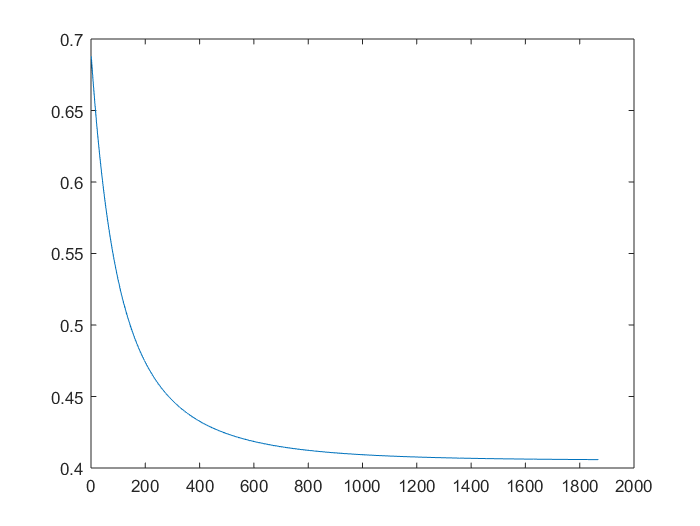
\includegraphics[width=0.45\textwidth]{figures/L1.png}}
		\subfigure[Decision Boundary]{
			\label{b1}
			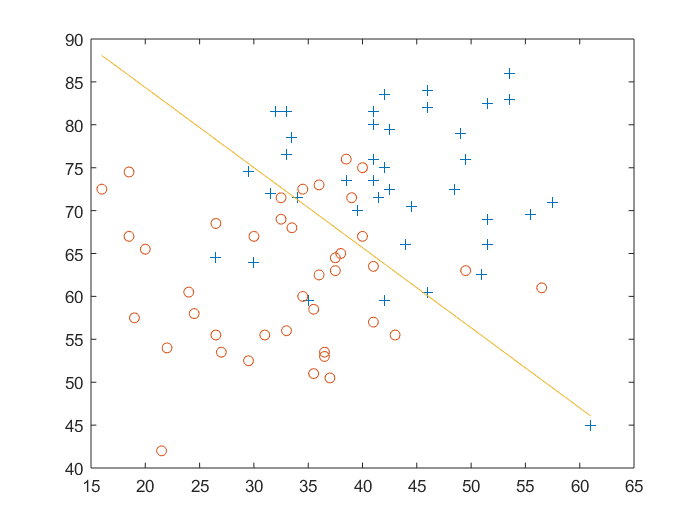
\includegraphics[width=0.45\textwidth]{figures/b1.png}}
		\caption{梯度下降法}
	\end{figure}

	\subsection{表格:}
	\begin{table}[H]
		\caption{第二问结果观察}
		\centering
		\linespread{1.5}
		\begin{tabular}{ccc}
			\toprule
			$c$  & 数据集1成功率 & 数据集2成功率 \\
			\midrule
			0.01 & 1             & 1             \\
			0.1  & 1             & 1             \\
			\bottomrule
		\end{tabular}
	\end{table}

	\subsection{图片:}
	\begin{figure}[H]
		\centering
		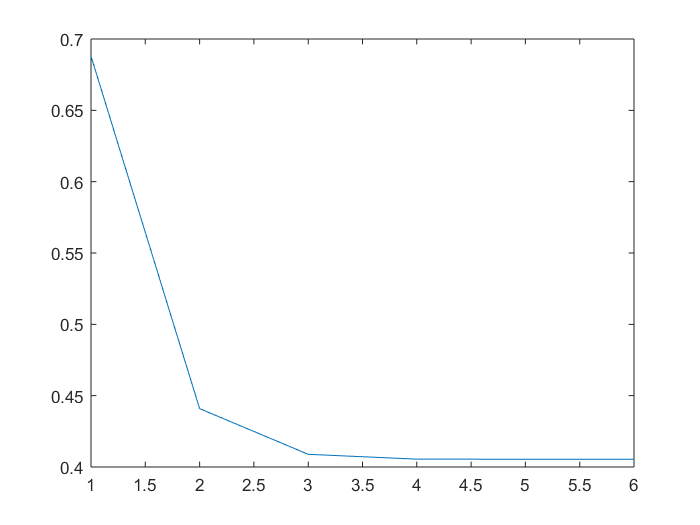
\includegraphics[width=0.7\textwidth]{figures/L2.png}
		\caption{开发团队}
	\end{figure}


\end{sduDocument}

\sduAppendix % 不需要附录二字注释掉这一行即可
\begin{lstlisting}[language=matlab]
	x = load("data2/ex2x.dat");
	y = load("data2/ex2y.dat");
	n = length(x);
	x = [ones(n, 1), x];
	stds = std(x);
	mu = mean(x);
	x(:, 2) = (x(:, 2) - mu(2)) ./ stds(2);
	x(:, 3) = (x(:, 3) - mu(3)) ./ stds(3);
\end{lstlisting}

\end{document}
